% Please make sure you insert your
% data according to the instructions in PoSauthmanual.pdf
\documentclass[a4paper,11pt]{article}
\usepackage{pos}
\usepackage{xcolor}
\usepackage{subcaption} % Modern package for subfigures
\usepackage{graphicx}   % Required for inserting images
\usepackage{float}
\usepackage{bbm}
\newcommand{\dd}{\mathrm{d}}
\newcommand{\wtil}[1]{\widetilde{#1}}
\newcommand{\deint}[2]{\dd^{#1}\;\!\!#2\;}
\newcommand{\br}[1]{\left\langle #1 \right |}
\newcommand{\kt}[1]{\left| #1 \right \rangle}
%
\newcommand{\Ntot}{N_{\mathrm{tot}}}
\newcommand{\LamSRG}{\Lambda_{\mathrm{SRG}}}
\newcommand{\LamNN}{\Lambda_{\mathrm{NN}}}
\newcommand\brktt[3]{\left< #1 \right| #2 \left| #3 \right>}
\newcommand{\bkt}[2]{\left \langle #1 |#2 \right \rangle}
\newcommand{\brkt}[2]{\left \langle #1 |#2 \right \rangle}
\newcommand{\eps}{\epsilon}
\newcommand{\cEFT}{$\chi$EFT}
\newcommand{\etal}{\textit{et al.}}
\newcommand{\Li}{\mathrm{Li}}
\newcommand{\LiS}{{}^{6} \mathrm{Li} }
\newcommand{\HeF}{{}^{4} \mathrm{He}}
\newcommand{\HeT}{{}^{3} \mathrm{He}}
\newcommand{\HThree}{{}^{3} \mathrm{H}}
\newcommand{\HT}{{}^{2} \mathrm{H}}
\newcommand\bv[1]{\vec{#1}}
\newcommand{\ques}[1]{\color{red}\textit{ #1 }\color{black}}
\newcommand{\comment}[1]{\color{blue}\small\textbf{ #1 }\color{black}\normalsize}
\newcommand{\com}[1]{\color{blue}\small\textbf{ #1 }\color{black}\normalsize}
\newcommand\ddfrac[2]{\frac{\displaystyle #1}{\displaystyle #2}}
\newcommand{\MeV}{\mathrm{MeV}}
\newcommand{\mev}{\mathrm{MeV}}
\newcommand{\fm}{\mathrm{fm}}
\newcommand{\fmin}{\mathrm{fm}^{-1}}
\newcommand{\rv}{\vec{r}}
\newcommand{\pv}{\vec{p}}
\newcommand{\ChiEFT}{$\chi$EFT}

\usepackage{ulem}
   \newcommand{\replace}[2]{\sout{\protect#1}\color{blue}#2\color{black}} 
   % provides underlines of various styles, good for commenting etc.
   % \uline{important}    underlined text
   \renewcommand{\emph}[1]{\textit{#1}}           % ulem overwrites def of
   % \dashuline{dashing}  dashed underline
   % \dotuline{dotty}     dotted underline
   % \uuline{urgent}      double-underlined text
   % \uwave{boat}         wavy underline 
   % \sout{wrong}         line drawn _through_ word
   % \xout{removed}       marked over (many "/////")
   \renewcommand{\emph}[1]{\textit{#1}}           % ulem overwrites def of \emph as \textit, so reinstate here
\title{Scattering Observables from Few-Body Densities and Application
in Light Nuclei}
%% \ShortTitle{Short Title for header}

\author*{Alexander Long}
% \author*[a]{Alexander Long}
\author{Harald W. Grie{\ss}hammer}

% \affiliation[a]{The George Washington University\\ Washington DC USA}
\affiliation{Institute for Nuclear Studies, Department of
Physics,\\George Washington University, Washington DC 20052, USA}
% \affiliation[a]{Institution,\\
%   Street number, City, Country}

% \affiliation[b]{Department, University,\\
% Street number, City, Country}

\emailAdd{alexlong@gwu.edu}
\emailAdd{hgrie@gwu.edu}
\abstract{
  The dynamics of scattering on light nuclei is well understood, but its
  calculation is numerically difficult using standard methods.
  Fortunately, using recent developments, the relevant quantities can
  be factored into a product of the $n$-body transition density
  amplitude (TDA) and
  the interaction kernel of a chosen probe.
  These TDAs depend only on the target, and not the
  probe; they are calculated once and stored.
  The kernels depend on only the probe and not the target; they can
  be reused for different targets.
  The calculation of transition densities becomes numerically
  difficult for $n\ge4$, but we discuss a solution through use of a
  similarity renormalization
  group transformation.
  This technique allows for extending the TDA method to $\LiS$.
  We present preliminary results for Compton scattering on $\LiS$ and
  compare with available data, anticipating an upcoming thorough studi~\cite{upcoming}.
  We also discuss ongoing extensions to pion-photoproduction and other reactions on $A\le6$ nuclei.
}

\FullConference{The 11th International Workshop on Chiral Dynamics (CD2024)\\
  26-30 August 2024\\
Ruhr University Bochum, Germany\\}

%% \tableofcontents

\begin{document}
\maketitle
\com{This is a comment, (for Dr.Griesshammer's use) $a^2$}
\ques{This is a question (for Alex's use)}
\section{Introduction}
\com{my proc will be very similar to 
    EPJ Web Conf. 303 (2024) 04002
        MENU 2023
e-Print:    2401.15673 [nucl-th] -- you might want to have a look.}
Effective Field Theories (EFTs) in nuclear physics provide a
framework for making precise predictions by employing only those
degrees of freedom that are most pertinent to the physical system
under consideration, rather than relying on the complete set of
intrinsic degrees of freedom present in the underlying theory
(typically quarks and gluons in nuclear and particle physics). In this work, we utilize Chiral
Effective Field Theory which adopts hadrons
as its fundamental degrees of freedom.
The present study is concerned with scattering probes off
light nuclei. To this end, the Transition Density \replace{approximation}{Amplitude} (TDA)
method was developed by Grie\ss hammer \textit{et al.} and de Vries
\textit{et al.}~\cite{hammer2020, Vries2024}. The TDA formalism
describes the interaction of a probe with an $A$-body target.
Consequently, the probe may interact with up to $A$ nucleons. The $n$ nucleons with which the probe
interacts are designated as \textit{active}, whereas the remaining
$A-n$ nucleons are referred to as \textit{spectators}. The
mathematical treatment of these two components is entirely distinct:
the active $n$ nucleons contribute to the $n$-body kernel, while the
spectator nucleons contribute to the $n$-body TDA.

The $n$-body kernel characterizes the interaction in reduced case
in which the probe interacts exclusively with the $n$-body
system. For example, the one-body kernel in Compton scattering
encompasses the same contributions as those arising in Compton
scattering off a single nucleon. This complete separation of the
contributions implies that if one has access to $a$ distinct kernels
and $b$ distinct TDAs, then a total of $ab$ different outcomes may be
generated. Figure~\ref{fig:onetwobod} provides an illustrative
example for the case $A=3$.

\begin{figure}[h]
  \begin{center}
    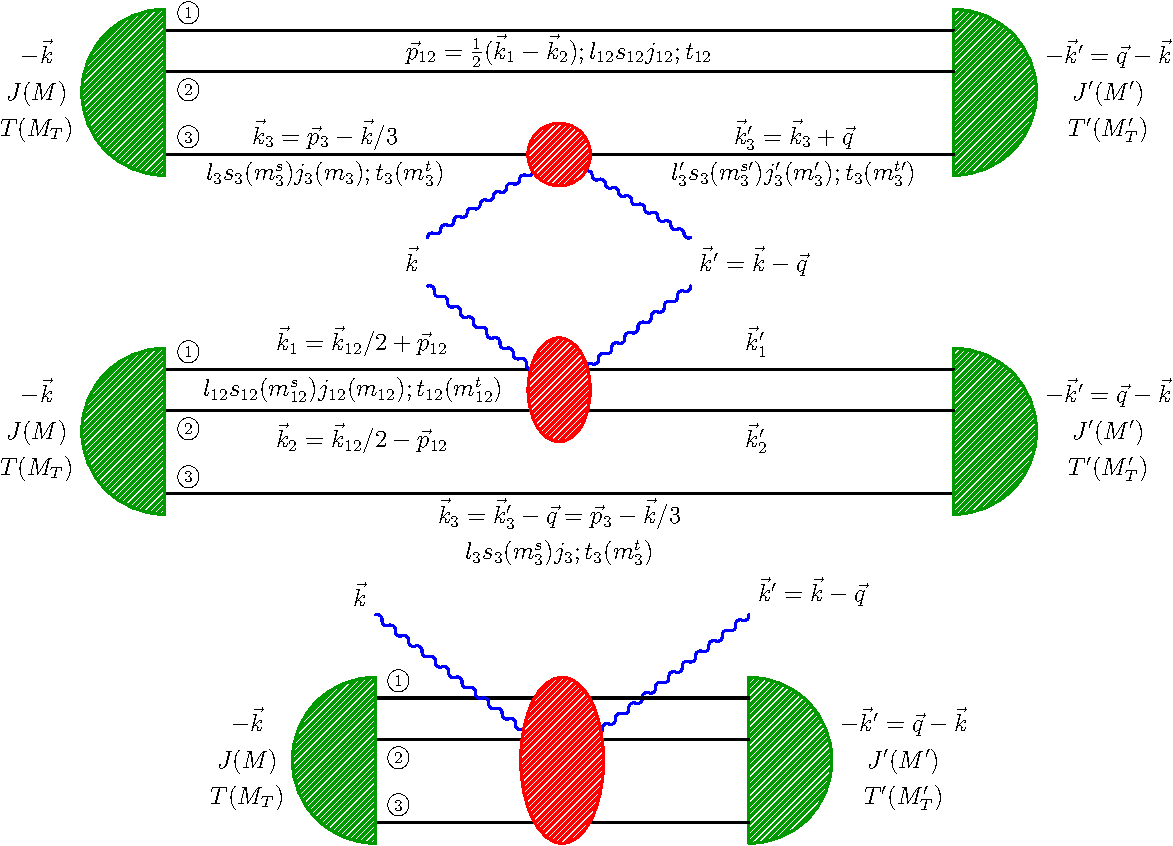
\includegraphics[scale=0.7]{kinematics3He.pdf}
    \caption{Kinematics in the center of mass frame and quantum
      numbers for an $A=3$ system in the case of Compton scattering.
      Generalization to other reactions only changes the kind of
      ingoing/outgoing probe. Generalization to $A>3$ would result in more internal lines
      representing the nucleons.
      Top: one-body processes $\hat{O}_1$ (one active nucleon, two spectators),
      center: two-body
      processes $\hat{O}_{2}$ (two active nucleons, one spectator), bottom: three-body processes
      $\hat{O}_{3}$ (all nucleons active, no spectators). Red represents the kernels; 
      everything else is represented by the densities.
      Green represents the wavefunction of the nucleons.
      From Grie{\ss}hammer \etal
    \cite{hammer2020}.\com{mention also momentum transfer, quantum numbers? Or just in text...}}
    \label{fig:onetwobod}
  \end{center}
\end{figure}

For scattering off an $A$-body nucleus, the total scattering
amplitude is given by \ques{you want a citation here but I think I am the first person to actually write this down. I can cite the $\HeT$ paper if you want.} \com{see 4He paper, eq. (2.5) -- but it's trivial}
\begin{align}
  A_{M}^{M^{\prime} }(\bv{k}, \bv{q})&=\binom{A}{1}\left\langle
  M^{\prime}\right|\hat{O}_{1}^{}(\bv{k}, \bv{q})\left|M\right
  \rangle + \binom{A}{2} \left\langle
  M^{\prime}\right|\hat{O}_{2}^{}(\bv{k}, \bv{q}) \left|
  M\right\rangle
  &+... + \binom{A}{A}\left\langle
  M^{\prime}\right|\hat{O}_{A}^{}(\bv{k}, \bv{q})\left|M\right
  \rangle
\end{align}

\begin{align}
  A_{M}^{M^{\prime} }(\bv{k}, \bv{q})&=
 \left\langle M^{\prime}\left|
  \binom{A}{1} \hat{O}_{1}(\bv{k}, \bv{q}) +
  \binom{A}{2} \hat{O}_{2}(\bv{k}, \bv{q}) +... + 
  \binom{A}{A} \hat{O}_{A}(\bv{k}, \bv{q})
  \right|M
  \right\rangle
\end{align}
where $\hat{O}_i$ is the $i$-body kernel, $M,M'$ is the spin projection of the
target nucleus, and there are
$\binom{A}{i}$ ways for a probe to hit $i$ nucleons. Fortunately,
$\chi$EFT provides a hierarchy of scales which predicts decreasing
contributions for higher order terms for probe energies greater than
$\sim 40 \MeV$.
Therefore, the 3-body contribution and higher is negligible at this
order\com{you have not yet talked about orders. Here or when you first talk about ChiEFT, you also should talk about a small dimless parameter -- maybe even write it down?}, and we simply use
\begin{equation}
  A_{M}^{M^{\prime} }(\bv{k}, \bv{q})=\binom{A}{1}\left\langle
  M^{\prime}\right|\hat{O}_{3}^{}(\bv{k}, \bv{q})\left|M\right
  \rangle + \binom{A}{2} \left\langle
  M^{\prime}\right|\hat{O}_{2}^{}(\bv{k}, \bv{q}) \left|
  M\right\rangle\nonumber\\
\end{equation}
In practice, this is enough for accuracy on roughly the 5\% level.
%%%%%%%%%%%%%%%%%%%%%%%%%%%%%%%%%%%%%%%%%%%%%%%%%%%%%%%%%%%%
\section{Kernels and Densities}
The one-body and two-body kernel must be considered separately.
Their form is different, and they require a one- and
two-body density respectively.
Symbolically, the matrix element $\hat{O}_1$ is:
\begin{align}
  \left\langle M^{\prime}\left|\hat{O}_{1}(\bv{k}, \bv{q})\right|
  M\right\rangle&=\sum_{\alpha \alpha^{\prime}} \int \mathrm{d}
  p_{12} p_{12}^{2} \mathrm{~d} p_{3} p_{3}^{2} \mathrm{~d}
  p_{12}^{\prime} p_{12}^{\prime 2} \mathrm{~d} p_{3}^{\prime}
  p_{3}^{\prime 2}
  \psi_{\alpha^{\prime}}^{\dagger}\left(p_{12}^{\prime}
  p_{3}^{\prime}\right) \psi_{\alpha}\left(p_{12} p_{3}\right)\nonumber \\
  &\times\left\langle p_{12}^{\prime}
  p_{3}^{\prime}\left[\left(l_{12}^{\prime} s_{12}^{\prime}\right)
    j_{12}^{\prime}\left(l_{3}^{\prime} s_{3}\right)
  j_{3}^{\prime}\right] J^{\prime} M^{\prime}\left(t_{12}^{\prime}
  t_{3}\right) T^{\prime} M_{T}\right| \hat{O}_{1}(\bv{k}, \bv{q})
  \label{onebodFull}\\
  &\qquad\qquad\left|p_{12} p_{3}\left[\left(l_{12} s_{12}\right)
  j_{12}\left(l_{3} s_{3}\right) j_{3}\right] J M\left(t_{12}
  t_{3}\right) T M_{T}\right\rangle.\nonumber
\end{align}\com{you introduce here a ton of symbols which are not explained, just to then immediately drop all of it and actually talk about eq (4). So what is the use of this eq?}
The central result is that up to relativistic corrections, this can
be written as:
\begin{align}
  \left\langle M^{\prime}\left|\hat{O}_{1}(\bv{k}, \bv{q})\right|
  M\right\rangle=\sum_{\substack{m_{3}^{s \prime}\,
  m_{3}^{s}\\m_3^t}}\hat{O}_{1}\left(m_{3}^{s \prime} m_{3}^{s},
  m_{3}^{t} ;  \bv{k}, \bv{q}\right) \rho_{m_{3}^{s \prime}
  m_{3}^{s}}^{m_3^{t} M_{T}, M^{\prime} M}(\bv{k}, \bv{q})\label{onebodyOrig}\;.
\end{align}
For full details see Grie{\ss}hammer \etal\cite{hammer2020}\com{and 4He paper}.
Here $\rho$, is the \textit{one-body transition density amplitude} (TDA)
for the nucleus which was discussed previously and can truly be
interpreted as the probability amplitude that nucleon $m_3^t$ absorbs
momentum $\bv{q}$, changes its spin projection from $m_s^3$ to
$m_s^{3'}$ and changes the spin-projection of the nucleus from $M$ to
$M'$\com{$M_T$ and $\vec{k}$ unexplained}; hence the name "Transition Density Amplitude". Its operator form is
\begin{equation}
  \rho_{m_{3}^{\prime} m_{3}^{s}}^{m_{3}^{t} M_{T}, M^{\prime}
  M}(\bv{k}, \bv{q})=\left\langle M^{\prime}\right.\left|s_{3}
  m_{3}^{s \prime}, t_{3} m_{3}^{t}\right\rangle
  \mathrm{e}^{\mathrm{i} \frac{2}{3} \bv{q} \cdot
  \bv{r}_{3}}\left\langle s_{3} m_{3}^{s}, t_{3}
  m_{3}^{t}\right|\left. M\right\rangle\label{onebodydens}.
\end{equation}
The two-body case works similarly, and results in
\begin{equation}
  \left\langle M^{\prime}\left|\hat{O}_{2}\right| M\right\rangle =
  \sum_{\alpha_{11}^{\prime}, \alpha_{12}} \int \mathrm{d} p_{12}\:
  p_{12}^{2} \mathrm{~d} p_{12}^{\prime}\: p_{12}^{\prime 2}\;
  O_{2}^{\alpha_{12}^{\prime} \alpha_{12}}\left(p_{12}^{\prime},
  p_{12}\right) \rho_{\alpha_{12}^{\prime} \alpha_{12}}^{M_{T},
  M^{\prime} M}\left(p_{12}^{\prime}, p_{12} ; \bv{q}\right)\label{twobody}\;.
\end{equation}
This is the two-body equivalent to \eqref{onebodyOrig}.
There is an expression analogous to \eqref{onebodFull} but it is
non-trivial and for our purposes non-enlightening.
This two-body density $\rho_{\alpha_{12}^{\prime}
\alpha_{12}}^{M_{T}, M^{\prime} M}$ is of course distinct
from the one-body density.
Moreover, just like the one-body case, it can also be interpreted as a
transition probability density amplitude \com{it's a prob amplitude, not already a prob}.
It depends on the incoming and outgoing quantum numbers
$\alpha_{12}$ and $\alpha_{12}'$ of the 1-2 system, and also on their initial and final
relative momenta $p_{12}$ and $p_{12}'$ of the two nucleons which are integrated over \com{it's not the 2 nucleons which are integrated over but their rel momenta. Need better formulation!}.
As a result, the file size for the two nucleon densities is approximately 20 MiB\com{I do not know this as abbreviation fro megabytes. I know MB or Mbyte}
per energy and angle, whereas those of the one
nucleon densities are on the order of a few KB.
Importantly, the densities $\rho$ can for a given momentum transfer $\vec{q}$ be computed directly from a nuclear
potential, such as the chiral SMS potential
\cite{Reinert2018}
without reference to the kernel $\hat{O}_1$ or $\hat{O}_{2}$.
%%%%%%%%%%%%%%%%%%%%%%%%%%%%%%%%%%%%%%%%%%%%%%%%%%%%%%%%%%%%%%%%%%%%%%%
\section{SRG Transformation}
Previous work using the TDA formalism has analyzed
$\HeT$ and $\HeF$
\cite{hammer2020, hammer4He}, but to extend this to $\LiS$ involves many-body
interactions which are much more complicated and computationally expensive.
To make the calculation of a TDA feasible for $A=6$, a
\textit{Similarity Renormalization Group} (SRG) transformation
is employed \cite{SRG, Furnstahl2013}.
This is of much experimental interest since $\LiS$ is a stable solid at room temperature and is
therefore relatively simple to conduct an experiment on, even to high precision, due to its relatively large
cross section and count rate.
There have been many\com{2 is not many} experiments on $\LiS$ \cite{60MeV,86MeV}, yet to date there is no theory prediction.
We seek to fill in this gap.
When using nuclear potentials, we approximate the nucleon-nucleon potential to be zero
beyond a certain cutoff $\LamNN$, and consequently
neglect contributions above this cutoff in our calculations.
In general, a nuclear potential, such as the chiral SMS \com{also de-acronymise S...M...S... (SMS)} potential does
not fall off rapidly at high momenta \cite{Reinert2018}.
As a result we would have to
extend the cutoff $\LamNN$ much further than is desirable\com{what is desirable? in eye of beholder. you give the actual argument: comp cost!}, which in turn
increases computational cost.
The SRG transformation is a unitary transformation that
shifts the relevant physics into the low-momentum
region, thereby lowering minimum effective $\LamNN$ in the SRG evolved space.
This, in turn, significantly improves the convergence rate of calculations for $A=6$ \com{you can add that it actually makes them possible}.
The SRG transformation can be thought of as a local averaging or
smoothing of the potential, resulting in decreased resolution
as the SRG is applied.\com{I like this sentence! Add that this does NOT compromise physics and only kills short-range fluctuation beyond EFT range of applicability?}
\begin{figure}[H]
  \centering
  \begin{subfigure}{0.45\textwidth}
    \centering
    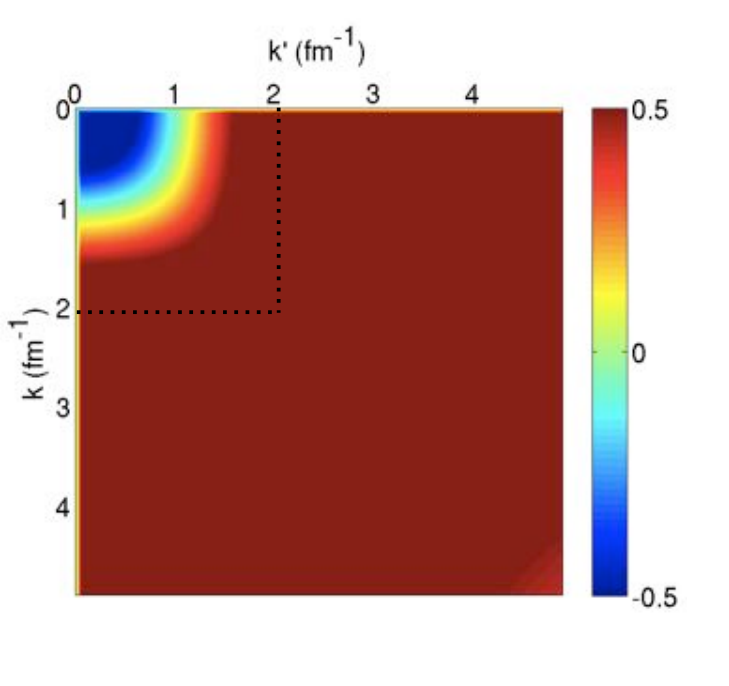
\includegraphics[width=\linewidth]{HighRes.png}
    \caption{High Resolution (before much SRG is applied) }
    \label{fig:highres}
  \end{subfigure}
  \hfill
  \begin{subfigure}{0.45\textwidth}
    \centering
    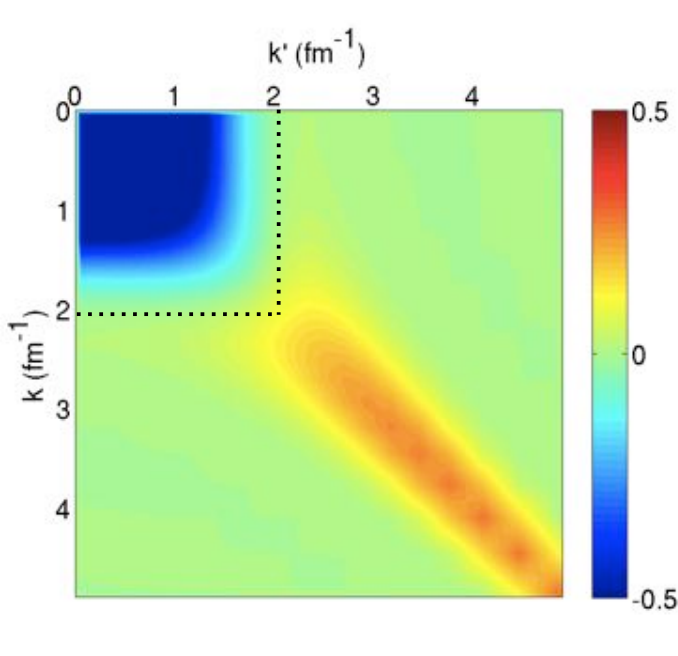
\includegraphics[width=\linewidth]{LowRes.png}
    \caption{Low Resolution (evolved)}
    \label{fig:lowres}
  \end{subfigure}
  \caption{Nuclear potentials $V(k,k')$. Figures from Kai Hebeler:
    ``Chiral Effective Field Theory and Nuclear Forces:
    overview and applications'' presentation at TALENT school at MITP
    2022, and modified with permission from
    Furnstahl \etal \cite{Furnstahl2013}.
  }
  \label{fig:SRGtransform}
\end{figure}
In the under-evolved, high resolution panel, fig.~\ref{fig:highres}, the potential does 
not go to zero rapidlyat large momenta, whereas it does once the
transformation is applied in the right panel, fig.~\ref{fig:lowres}. As a
result, a cutoff can be made at $\LamNN=2 \mathrm{fm}^{-1}$ without
losing much accuracy, whereas the under-evolved potential required at least $\LamNN=5 \mathrm{fm}^{-1}$.
The time complexity is at a minimum proportional to the number of array elements
present, therefore we gain at least a factor of $(5/2)^2=6.25$ in efficiency;
in practice the gains are even higher because near-zero values of the potential at parge momenta means sparser grids can be used there.\com{I added the "killer" sentence. Don't forget that you need to TELL the reader what to see and what to think. You CANNOT rely that they will make the inferences you think are trivial.}

\com{where are you talking about the NCSM as a method to compute 6Li?}

The SRG transformation is essential, but it also creates a
change in the physical meaning of the free variables.
In fact, any unitary transformation ($U^\dag U =\mathbbm{1}$) also transforms the coordinates:
\begin{align}
  \br{p'}V\kt{p} 
  = \br{p'} U^\dag U V U^\dag U \kt{p}
  = \br{p'} U^\dag\left( U V U^\dag\right)\;U
  \kt{p}
  = \br{\widetilde{p}\,'} V_{eff}
  \kt{\widetilde{p}}=V_{eff}(\widetilde{p},\widetilde{p}\,')
\end{align}
So referring to the free variables in an SRG-transformed potential as
``momenta'' is, to some extent, incorrect.
They do not represent physical states  in the sense that they are not eigenstates to physical momenta.
The Lagrangeans that generate the Feynman diagrams in the kernel, however,
depend on physical momenta, and therefore we cannot directly use an SRG
evolved potential in the non-SRG evolved kernel.
To solve this, previous work with SRG transformations has transformed the
Lagrangeans - and therefore the kernels - into the SRG evolved space
as well\ques{get citation}.
However, in the context of the density formalism this would mean adding SRG
dependence into the kernel, thereby breaking kernel-density independence. \com{be explicit why this is bad: one has tto transform the kernel with the same SRG every time one applies a kernel with the SRGd density: cn lead to mismatches, more work for user,... (you elaborated on that in your talk at ChiDyn!)}
Additionally, the SRG transformation can take many different forms \cite{SRG, Furnstahl2013};
we wish to allow for these developments
without having to re-write the kernel code.
Therefore we \replace{have chosen}{developed a method} to apply an inverse
transformation to the densities \cite{XiangXiang}. \com{be more explicit: therefore, we chose to first perform the SRG, then compute the densities via the SRG potential, and then apply the inverse SRG trafo to find the densities without SRG.}

The SRG evolution has parameters that must be fine-tuned, but this
allows for uncertainty estimation.
In particular, one must solve for the nucleus wavefunction; 
to this end an expansion in the harmonic oscillator basis is used \cm{this is not SRG but NCSM -- mention, reference, de-acronymise! -- see above}.
When expanded to infinite order, this basis forms a complete set,
however, we truncate this expansion by including harmonic oscillator excitations up to $\Ntot$.
Additionally, the harmonic oscillator basis has a characteristic
width, denoted by $\omega_H$, and finally, the parameter $\LamSRG$
represents the SRG evolution of the potential, as seen in figure
\ref{fig:SRGtransform}. $\LamSRG=\infty$ corresponds to no evolution.
All of these parameters affect the resulting cross-section. \com{why? is this the moment to mention induced many-body interactions in SRG? Or later?}
We note that uncertainty decreases monotonically\com{are you sure it's monotonically?} with increasing
$\Ntot$, and at $\Ntot=\infty$ the associated uncertainty goes to zero.

\com{this is a comment on the next paragraphs. You state a thesis like a mathematician states a theorem, and then you provide evidence for the thesis (like a proof). I think a Physicist's reaction is "why does he say this?" -- nd then as to read to the end to see that this is actually covered by the facts. I propose to write this starting from the facts (SRG is not unitary, so we must check. Do 4He to test - -we see small deviations...}

Applying a stronger\com{"longer"?  "evolving to smaller $\LamSRG$"} SRG evolution (lower $\LamSRG$) to the potential results in larger
induced many-body forces \com{see above: yes, but elaborate in 1/2 sentence why that is!: your SRG is actually not quite unitary because we leave induced A>3 boydy interactions out.}; however, we show in figure \ref{fig:SRGConverge4He} the
effect of this uncertainty is small \com{in 4He, where the numerical cost is small enough that we can compare potentials with and without SRG evolution}.
These induced forces exist because due to the cutoff $\LamNN$ the SRG transformation
is only approximately unitary. \com{this explanation comes too late.}
Fortunately, when the TDA is calculated we also gain access to the
binding energy of the simulated system.
From this, we can estimate \replace{required}{optimal} values for $\omega_H$ and
$\Ntot$ \om{right now, we take the "optimal" omegaH to get a good binding energy but make Ntotmax as large as possible. So we do not optimise Ntotmax} by comparing the experimental binding energy to the computed
binding energy.
In order to gain confidence we first applied this methodology 
to $\HeF$, where we can compare SRG and non-SRG evolved results. 
With this completed we have now moved to $\LiS$ where we only have access to 
the SRG evolved form. \com{here or later: we will carefully investigate to which extet different LambdaSRG extrapolate to compatible values...}
\begin{figure}[H]
  \begin{center}
    \includegraphics[width=\linewidth]{
    4HeCrossSection.rel-dev-SRG-vs-nonSRG.chiralsmsN4LO+3nfN2LO-Λ550.Odelta2.pdf}
    \caption{$\HeF$\, Compton scattering SRG convergence \com{discuss deviation between "exact" and "SRGd" results: exists because of..., but small, so induced manybdoy small.}}
    \label{fig:SRGConverge4He}
  \end{center}
\end{figure}

\com{needs text}
\begin{equation}
  \text{``Relative deviation, (Rel. deviation) of $A$ from $M$''}:=
  \frac{A}{M}-1
\end{equation}
In figure \ref{fig:SRGConverge4He}, we see the effectiveness of the
results in the $\HeF$ case.
We expect the deviation to decrease as $N$ increases, and importantly
for our analysis, this shows what value of $N$ is required.
The small error present at high $\Ntot$ is present do to the induced many body forces.

\begin{figure}[H]
  \centering
  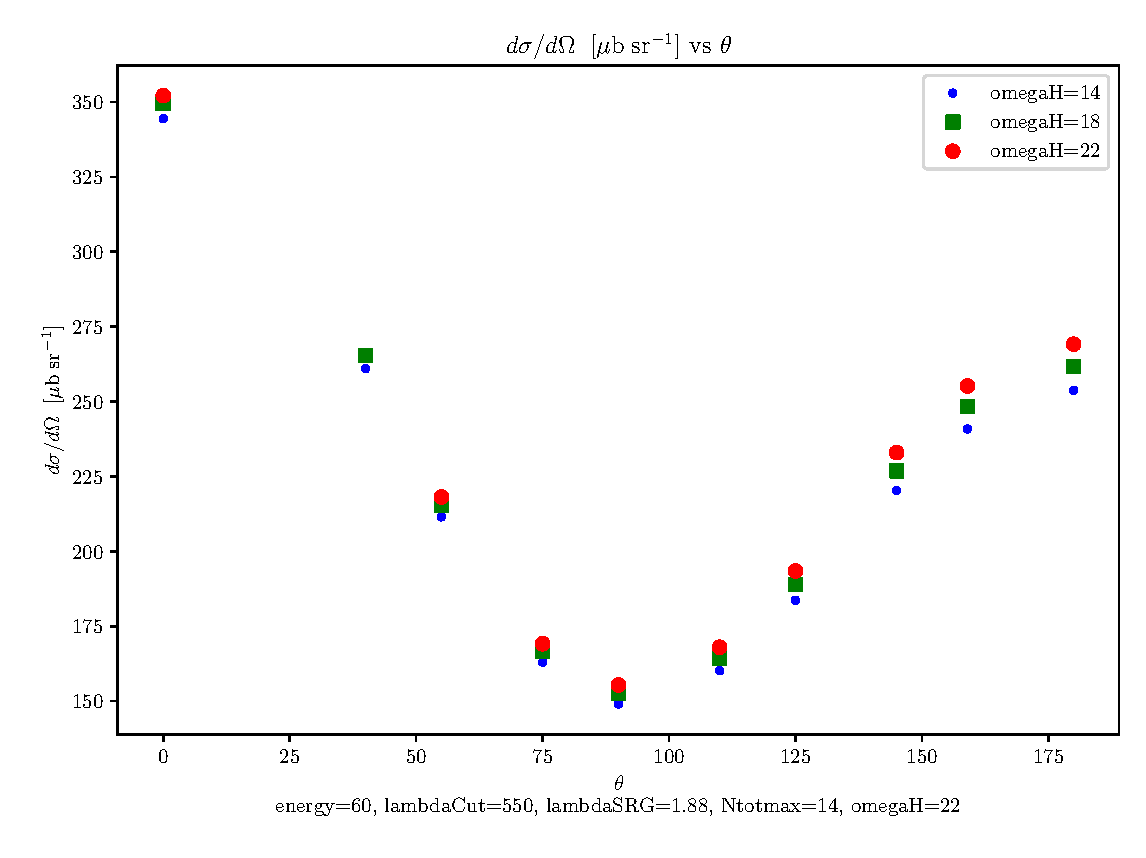
\includegraphics[scale=0.5]{6Li-omegaH-vary.pdf}
  \caption{Caption}
  \label{fig:label1}
\end{figure}

\com{from here on, presentation needs a lot more verbiage and detail -- but I guess you know that}

\com{discuss input: kernels same as in 34He (reference), central values of polarisabilities same as there (aae central values of most recent extractions, reference). Comparison to HIGS data is good/bad/undecided. Will study convergence in detail. Here assumed overall 10\% error as in 34He from potential/cutoff variations plus order-by-order convergence plus numerics plus extrapolations in LambdaSRG/Ntotmax/omegaH,... get inspired by 1-paragraph summary in 4He paper. }

\begin{figure}[H]
  \centering
  %\includegraphics[width=\linewidth]{file_path}
  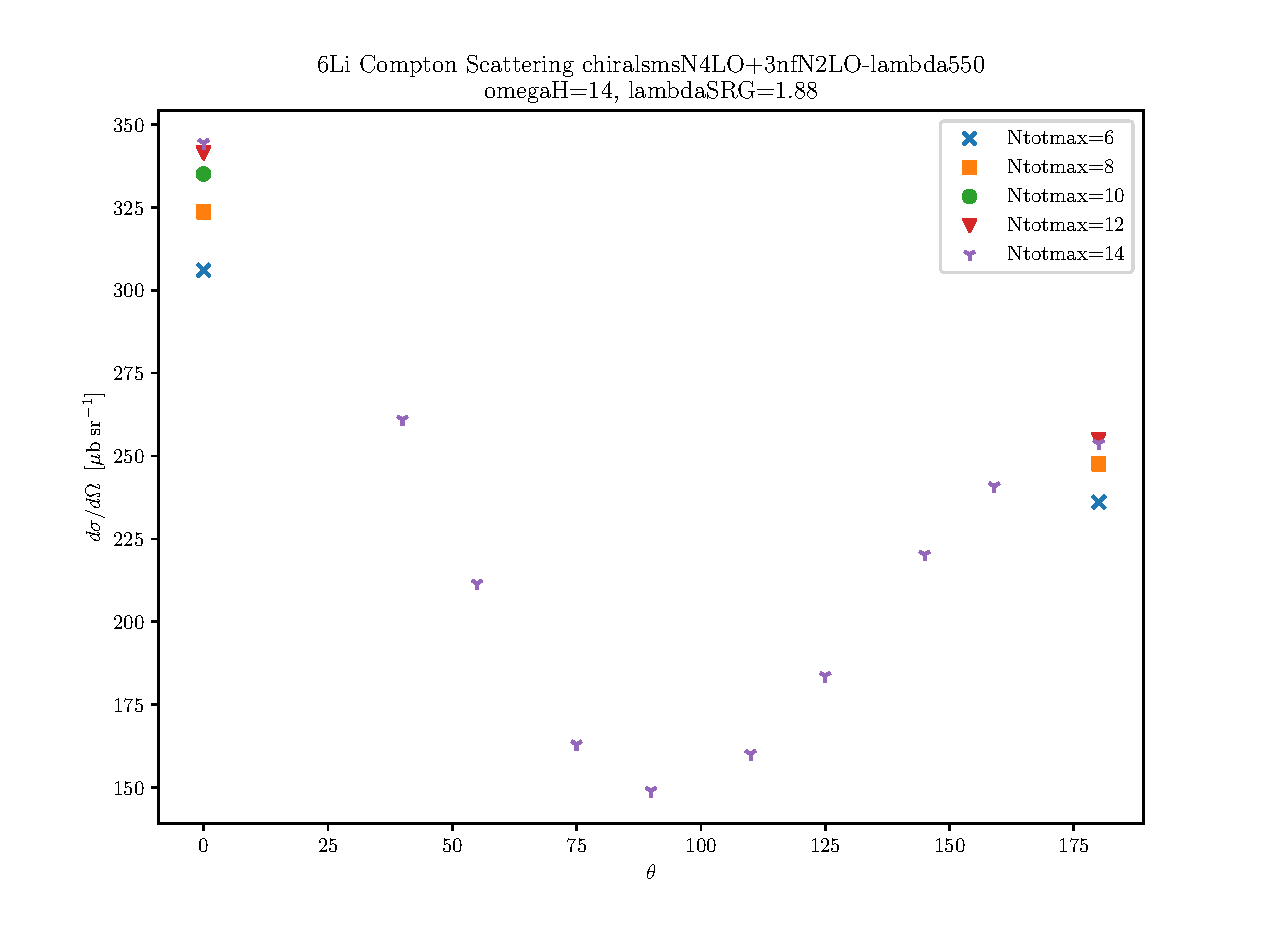
\includegraphics[scale=0.5]{6Li-Ntotmax-vary-omegaH14.pdf}
  \caption{Caption}
  \label{fig:label2}
\end{figure}
%%%%%%%%%%%%%%%%%%%%%%%%%%%%%%%%%%%%%%%%%%%%%%%%%%%%%%%%%%%%%%%%%%%%%
\section{Using TDAs in different processes}
With the TDAs calculated for Compton scattering, we now wish to recycle them for new processes.
In particular pion-photoproduction, and
pion scattering are of interest.
Fortunately their kernels share remarkable similarity since if one ignores the type of incoming/outgoing 
particle the processes are topologically identical.
\begin{figure}[H]
\centering
%\includegraphics[width=\linewidth]{file_path}
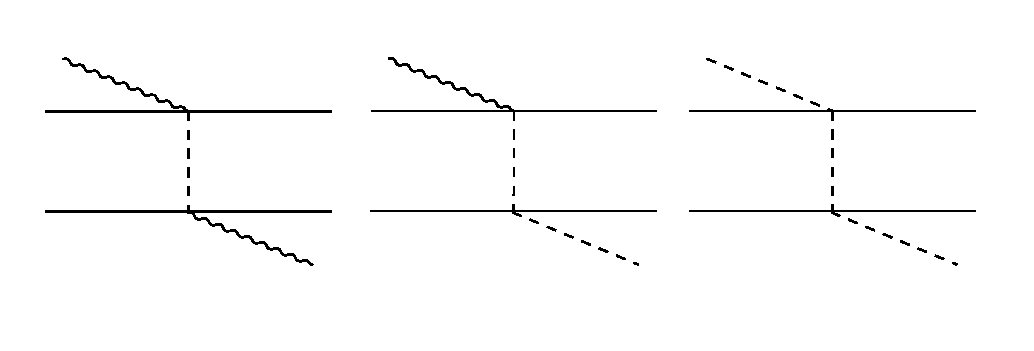
\includegraphics[scale=0.5]{KernelSim.pdf}
\caption{Topologically identical diagrams in Compton scattering, pion-photoproduction, and pion scattering \com{twobody only -- add onebody?}}
\end{figure}
\subsection{Pion-Photoproduction}
For the pion-photoproduction one-body kernel, we use the results from
single-nucleon scattering, $\gamma N \to \pi N$ which has
been studied extensively both in CHiEFT and phenomenologically \cite{pionphoto,
Rijneveen2021,Workman2012,Briscoe2023}.
Its differential cross section can be decomposed into the
electric and magnetic multipoles $E_{l\pm}, M_{l\pm}$ \cite{pionphoto}.
Over the years, many experiments have measured
these multipoles to high order and with good precision
\cite{multipolePionPion}.
The resulting scattering matrices $\mathcal{M}$ are exactly what
enters as $\hat{O}_1$ in equation (\ref{onebodyOrig}).
This approach solves a significant problem since the calculation of
the one-body pion-photoproduction kernel
to high accuracy directly from Feynman diagrams requires including many terms
in the chiral expansion due to the proximity of the $\Delta(1232)$ resonance at $\sim 200\MeV$. \com{That has been reported by Rijneeven et al \cite{Rijneveen2021}, and we add that to our stuff as well (I get tired, so no nice wording here).}


The two-body contributions do not easily decompose into multipoles, \replace{therefore}{so} we perform the calculation through expansions
in the chiral Lagrangean through \com{"through" twice in same sentence} calculation of Feynman diagrams. com{you MUST inlcude here that this 2B kernel is well-known, wee Weinberg, Beane, etc! YOu will be hung when you do not refernce these in a talk/paper because this process was absolutely instrumental to make ChiEFT credible. The non-chiral attempts all got the magnitude of the twobody effect wrong and laughed about the CHiEFT number -- until MAMI did the deuteron experiment, and that found the ChiEFT value. So this is a "milestone" kernel!! YOU write below about the Beane kernel -- so here too!}
It is likely this will lead to large uncertainties, as in the one-body case. \com{I would cut the preceding. We can do order-by-order error estimate -- but not here. Don;t be defensive if you do not yet know the result!}
At threshold energy, this reaction kernel has been analyzed by
Lenkewitz \etal \cite{L2011, L2013}.
We now have a numerically stable result for $\HeT$ and seek to extend
this approach to new targets.
\ques{Include some numbers, need to discuss with you uncertainty analysis.} \com{yes!!!!}
\subsection{Pion scattering and other reactions}
Beane \etal have developed the pion-pion \com{yu always write pion-pion scattering, YOu scatter one pion: it comes in and then goes out again. pion-pion makes it sound as if you scatter two pions on each other, or two pions on a nucleus.} kernel at threshold for both
one-body and two-body interactions \cite{Beane2003}.
We \replace{may}{anticipate to} extend this analysis to finite energy \com{in <target nuclei>}.
Once the pion-photoproduction and pion-pion scattering kernels have
successfully been developed, we will be able to calculate all of
these reactions on previously analyzed targets in the density
formalism since we already have produced \com{most of} the TDAs required.
In particular, we will calculate all of these reactions with the
targets $\HThree$, $\HeT$, $\HeF$, and $\LiS$. \com{relocate to 2 sentences prior}

\com{why is this interesting? first study (?) of ChiSym in these processes at heavier nucei. But beware Braun PhD thesis: maybe cite to reflect literature?}

%%%%%%%%%%%%%%%%%%%%%%%%%%%%%%%%%%%%%%%%%%%%%%%%%%%%%%%%%%%%%%%%%%%%%%%%%%%%%%%%%%%%%%
\section{Conclusion}
We \replace{have developed and demonstrated}{described} \com{this is a proceeding, and you gave an overview and talked about upcoming work.} a comprehensive framework for
computing scattering observables in light nuclei by factorizing the
full amplitude into target‐dependent few-body transition density
amplitudes (TDAs) and probe‐dependent interaction kernels\com{, summarising and expanding work in refs\cite{}}.
This separation allows us to treat the nuclear structure and the
reaction mechanism independently, thereby streamlining the
calculation of observables.
The central \sout{achievement of this work}\com{again: you report on ongoing work.} is the successful extension of
the density formalism to heavier targets like $\LiS$ by incorporating a
similarity renormalization group (SRG) transformation.
The SRG not only accelerates the convergence of our calculations by
lowering the effective momentum cutoff, but—when combined with an
appropriate inverse transformation of the densities—also preserves
the kernel–density independence that is crucial for the versatility
of our approach.
Furthermore, we have presented \com{you could write sth like "we presented first and preliminary results on.... Compton 6Li, summarising some key findings of an upcoming publication \cite{} which will also address pols sensitivity, detailed convergence study, detailed study of numerical and theory uncertainties, of world peace,...} the computation of Compton scattering on $\LiS$ which agrees
well with data, and we have outlined the ongoing extension of the formalism to other
reactions, such as pion-photoproduction and pion\sout{-pion} scattering \com{on 34He, 6Li and possibly other light nuclei} \cite{cite your thesis proposal and upcoming publication!}. The
ability to plug in different reaction kernels into the same TDA
framework\com{, and vice versa,} not only enhances the predictive power of our approach but
also paves the way for a unified treatment of various scattering
processes in \com{a wide range of} few-body systems.
Ultimately, this framework provides a promising route toward
high-precision theoretical predictions, deepening our understanding
of nuclear dynamics in light nuclei. \com{very nice final sentence -- catchy, worldly}

%%%%%%%%%%%%%%%%%%%%%%%%%%%%%%%%%%%%%%%%%%%%%%%%%%%%%%%%%%%%%%%%%%%%%%%%%%%%%%%%%%%%%%
\com{acknowledgments: Andreas+, supercomputer usage, DOE and DFG grants -- see 4He paper}
%%%%%%%%%%%%%%%%%%%%%%%%%%%%%%%%%%%%%%%%%%%%%%%%%%%%%%%%%%%%%%%%%%%%%%%%%%%%%%%%%%%%%%
\begin{thebibliography}{99}
  \bibitem{hammer2020}
  H. W. Grie{\ss}hammer, J. A. McGovern, A. Nogga, and D. R.
  Phillips, ``Scattering Observables from One- and Two-body
  Densities: Formalism and Application to $\gamma^3$ Scattering,''
  \textit{Few-Body Systems}, vol. 61, no. 4, Nov. 2020. DOI:
  \href{https://doi.org/10.1007/s00601-020-01578-w}{10.1007/s00601-020-01578-w}.

  \bibitem{Reinert2018}
  P. Reinert, H. Krebs, and E. Epelbaum, ``Semilocal momentum-space
  regularized chiral two-nucleon potentials up to fifth order,''
  \textit{The European Physical Journal A}, vol. 54, no. 5, May 2018.
  DOI:
  \href{http://dx.doi.org/10.1140/epja/i2018-12516-4}{10.1140/epja/i2018-12516-4}.
  \bibitem{hammer4He}
Grießhammer, H.W., Liao, J., McGovern, J.A. et al. Compton scattering on 
 with nuclear one- and two-body densities. Eur. Phys. J. A 60, 132 (2024). https://doi.org/10.1140/epja/s10050-024-01339-x
\href{https://arxiv.org/abs/2401.16995}{arXiv:2401.16995}.

\bibitem{SRG}
S. Szpigel and R. J. Perry, ``The Similarity Renormalization Group,'', Quantum Field Theory: A Twentieth Century Profile,
Sep. 2000. \href{https://doi.org/10.48550/arXiv.hep-ph/0009071}{https://doi.org/10.48550/arXiv.hep-ph/0009071}
  
  \bibitem{pionphoto}
  R. L. Walker, ``Phenomenological Analysis of Single-Pion
  Photoproduction,'' \textit{Phys. Rev.}, vol. 182, no. 5, pp.
  1729--1748, Jun. 1969. DOI:
  \href{https://link.aps.org/doi/10.1103/PhysRev.182.1729}{10.1103/PhysRev.182.1729}.

  \bibitem{multipolePionPion}
  R. L. Workman, M. W. Paris, W. J. Briscoe, and I. I. Strakovsky,
  ``Unified Chew-Mandelstam SAID analysis of pion photoproduction
  data,'' \textit{Phys. Rev. C}, vol. 86, no. 1, p. 015202, Jul.
  2012. DOI:
  \href{https://link.aps.org/doi/10.1103/PhysRevC.86.015202}{10.1103/PhysRevC.86.015202}.

\bibitem{Rijneveen2021}
N. Rijneveen, A. M. Gasparyan, H. Krebs, and E. Epelbaum, ``Pion photoproduction in chiral perturbation theory with explicit treatment of the $\Delta(1232)$ resonance,'' \textit{Phys. Rev. C}, vol. 106, no. 2, p. 025202, Aug. 2022. DOI: \href{https://link.aps.org/doi/10.1103/PhysRevC.106.025202}{10.1103/PhysRevC.106.025202}.

  \bibitem{L2011}
  M. Lenkewitz, E. Epelbaum, H.-W. Hammer, and U.-G. Meißner,
  ``Neutral pion photoproduction off $^3$H and $^3$He in chiral
  perturbation theory,'' \textit{Physics Letters B}, vol. 700, no. 5,
  pp. 365–368, Jun. 2011. DOI:
  \href{http://dx.doi.org/10.1016/j.physletb.2011.05.036}{10.1016/j.physletb.2011.05.036}.

  \bibitem{L2013}
  M. Lenkewitz, E. Epelbaum, H.-W. Hammer, and U.-G. Meissner,
  ``Threshold neutral pion photoproduction off the tri-nucleon to
  $O(q^4)$,'' \textit{The European Physical Journal A}, vol. 49, no.
  2, Feb. 2013. DOI:
  \href{http://dx.doi.org/10.1140/epja/i2013-13020-1}{10.1140/epja/i2013-13020-1}.

  \bibitem{86MeV}
  L. S. Myers, M. W. Ahmed, G. Feldman, A. Kafkarkou, D. P.
  Kendellen, I. Mazumdar, J. M. Mueller, M. H. Sikora, H. R. Weller,
  and W. R. Zimmerman, ``Compton scattering from $^{6}\mathrm{Li}$ at
  86 MeV,'' \textit{Phys. Rev. C}, vol. 90, no. 2, p. 027603, Aug.
  2014. DOI:
  \href{https://link.aps.org/doi/10.1103/PhysRevC.90.027603}{10.1103/PhysRevC.90.027603}.

  \bibitem{60MeV}
  L. S. Myers, M. W. Ahmed, G. Feldman, S. S. Henshaw, M. A. Kovash,
  J. M. Mueller, and H. R. Weller, ``Compton scattering from $^{6}$Li
  at 60 MeV,'' \textit{Phys. Rev. C}, vol. 86, no. 4, p. 044614, Oct.
  2012. DOI:
  \href{https://link.aps.org/doi/10.1103/PhysRevC.86.044614}{10.1103/PhysRevC.86.044614}.

  \bibitem{Beane2003}
  S. R. Beane, V. Bernard, E. Epelbaum, U.-G. Meißner, and D. R.
  Phillips, ``The S-wave pion–nucleon scattering lengths from pionic
  atoms using effective field theory,'' \textit{Nuclear Physics A},
  vol. 720, no. 3–4, pp. 399–415, Jun. 2003. DOI:
  \href{http://dx.doi.org/10.1016/S0375-9474(03)01008-X}{10.1016/S0375-9474(03)01008-X}.

  \bibitem{Workman2012}
  R. L. Workman, M. W. Paris, W. J. Briscoe, and I. I. Strakovsky,
  ``Unified Chew-Mandelstam SAID analysis of pion photoproduction
  data,'' \textit{Phys. Rev. C}, vol. 86, no. 1, p. 015202, Jul.
  2012. DOI:
  \href{https://link.aps.org/doi/10.1103/PhysRevC.86.015202}{10.1103/PhysRevC.86.015202}.
  \bibitem{Briscoe2023}
  W. J. Briscoe, A. Schmidt, I. Strakovsky, R. L. Workman, and A.
  \ifmmode \check{S}\else \v{S}\fi{}varc, ``Extended SAID
  partial-wave analysis of pion photoproduction,'' \textit{Phys. Rev.
  C}, vol. 108, no. 6, p. 065205, Dec. 2023. DOI:
  \href{https://link.aps.org/doi/10.1103/PhysRevC.108.065205}{10.1103/PhysRevC.108.065205}.
  \bibitem{Furnstahl2013}
  R. J. Furnstahl and K. Hebeler, ``New applications of
  renormalization group methods in nuclear physics,'' \textit{Reports
  on Progress in Physics}, vol. 76, no. 12, p. 126301, Nov. 2013.
  DOI:
  \href{http://dx.doi.org/10.1088/0034-4885/76/12/126301}{10.1088/0034-4885/76/12/126301}.
  \bibitem{XiangXiang}
  X.-X. Sun, H. Le, A. Nogga, and U.-G. Meißner, in preparation (2025).

  \bibitem{Vries2024}
  J. de Vries, C. Körber, A. Nogga, et al., ``Dark matter scattering
  off He in chiral effective field theory,'' \textit{Eur. Phys. J.
  C}, vol. 84, p. 1138, 2024. DOI:
  \href{https://doi.org/10.1140/epjc/s10052-024-13477-z}{10.1140/epjc/s10052-024-13477-z}.
\end{thebibliography}

\end{document}
